
\section{Unity 3D: Modelling the Environment}\label{appendix:unity3d-environment-modeling}
\begin{figure}[!ht]
        \centering
        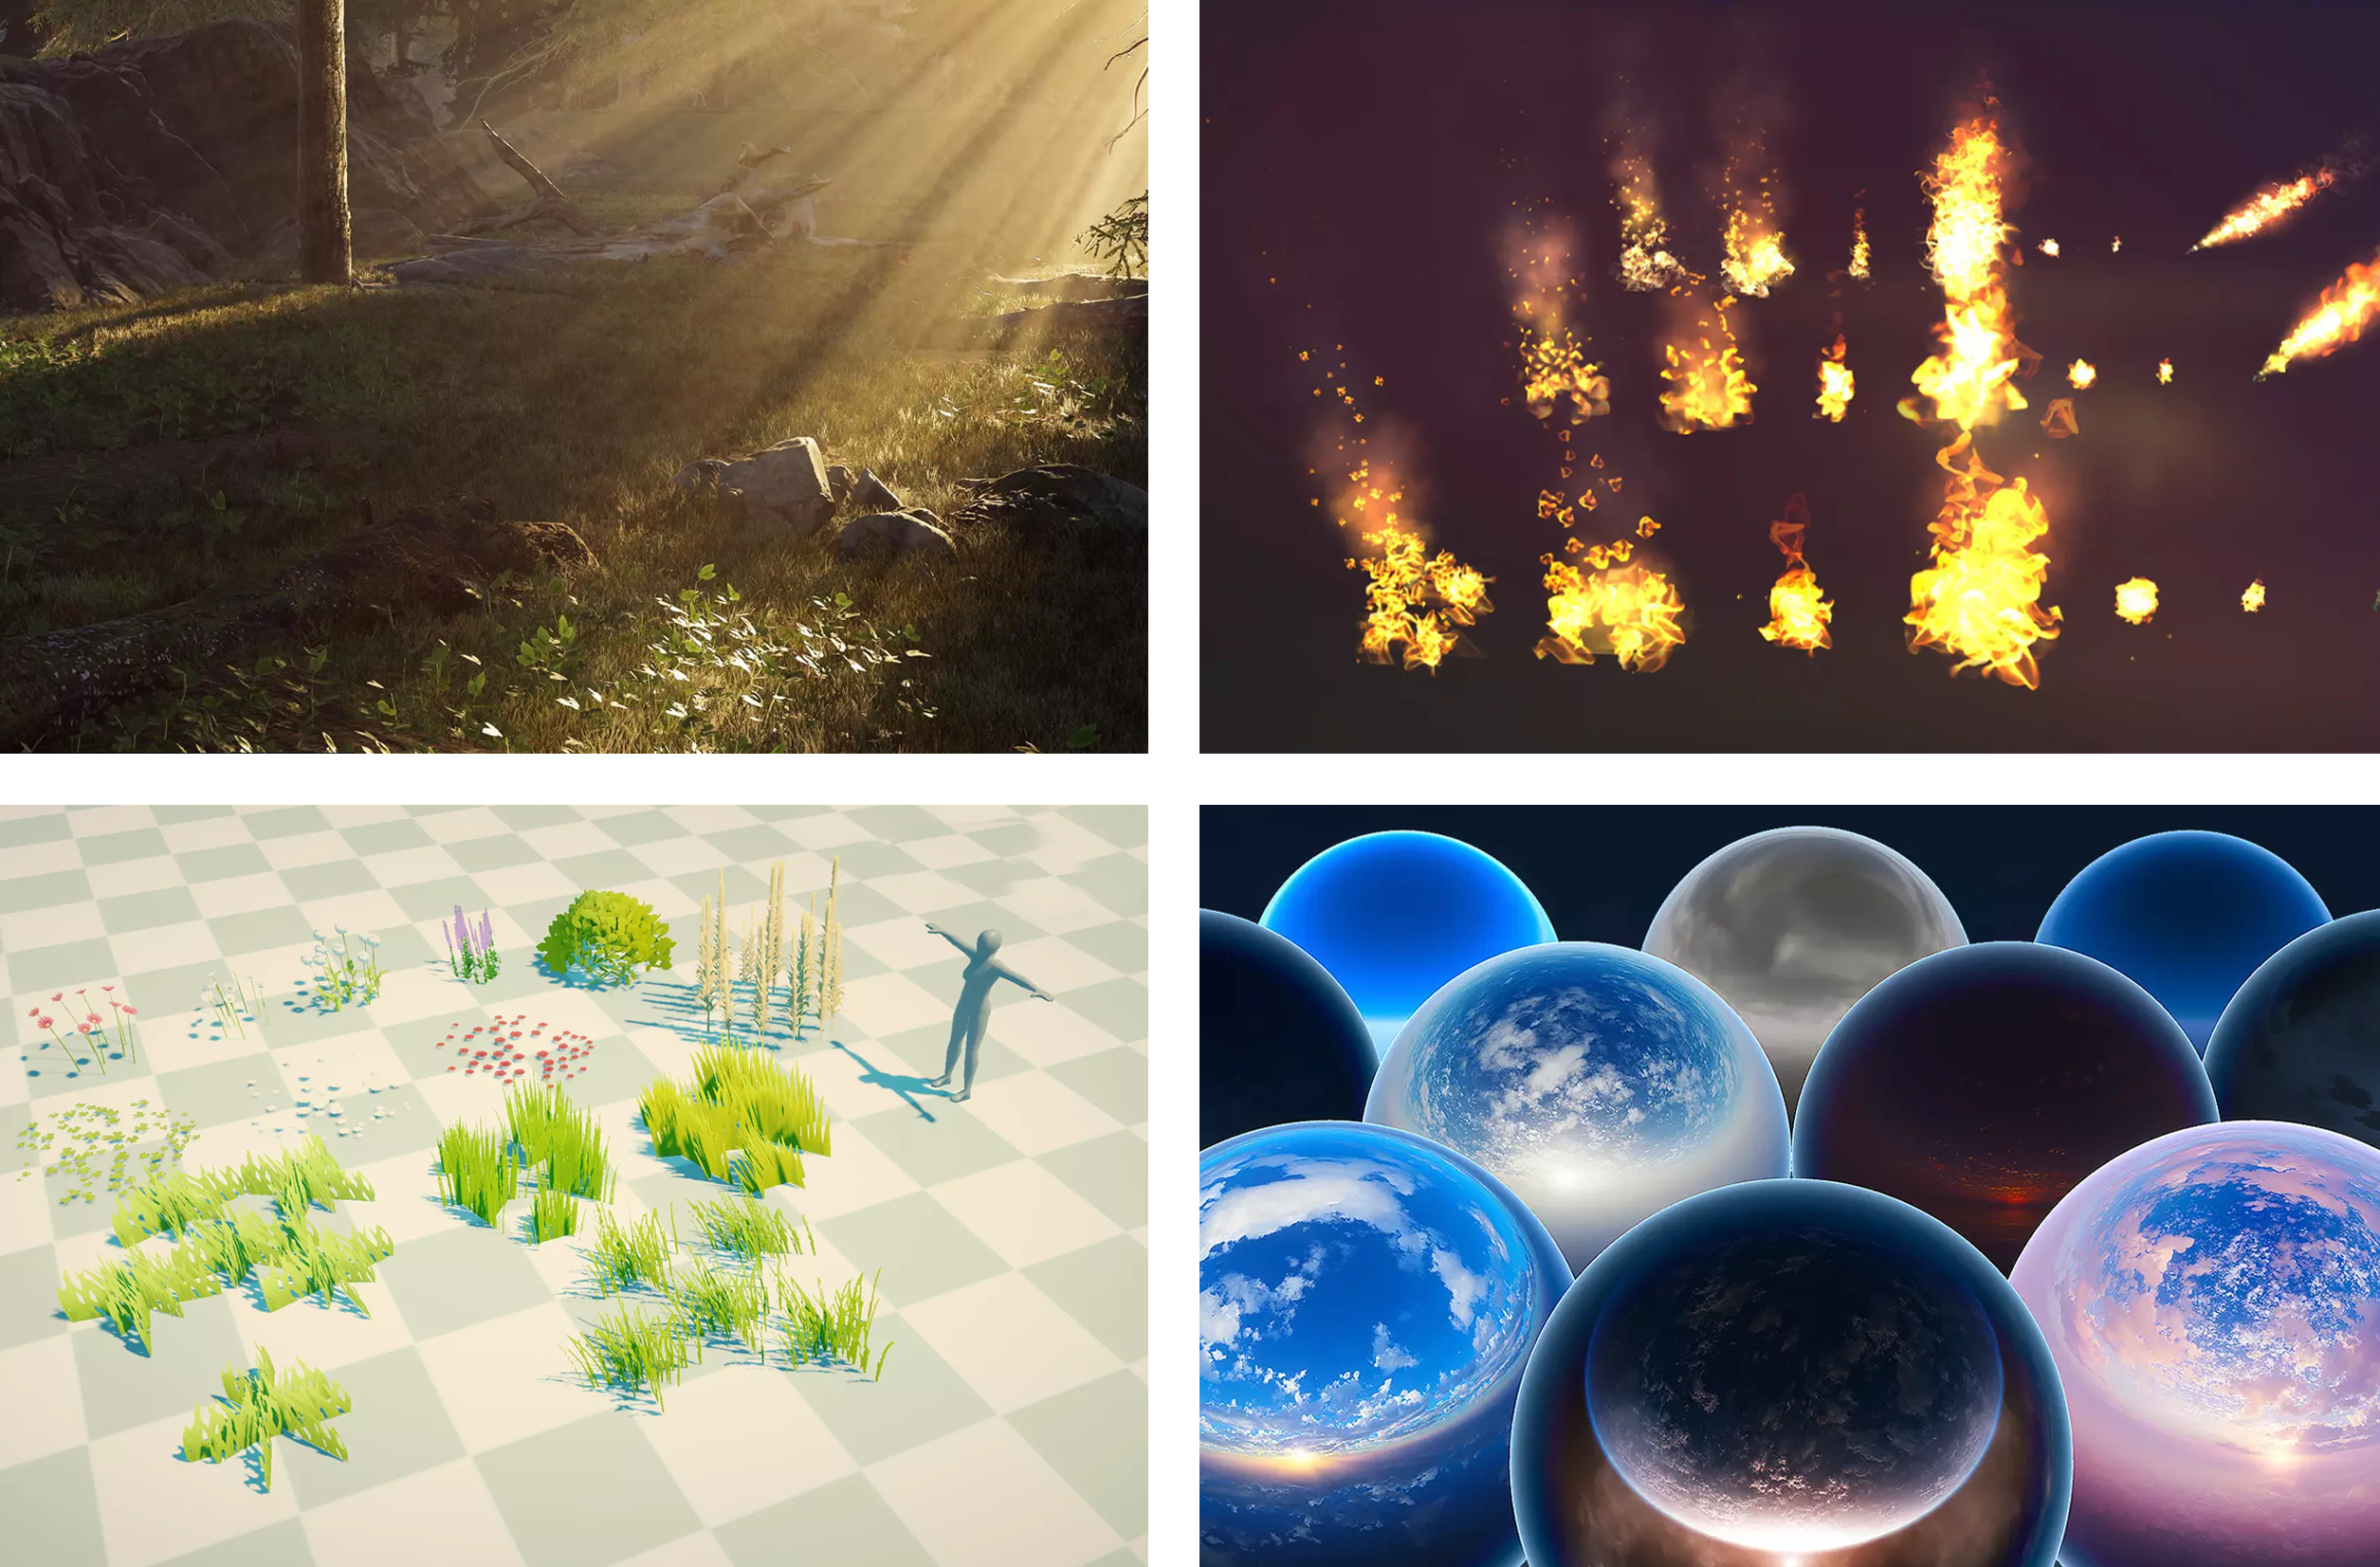
\includegraphics[width=0.8\textwidth]{images/unity-assets.png}
        \caption{Diverse Unity 3D Assets used to model 3D environments for the learning agent \cite{unityAssetStore}. Wireframe Shader (top left), Drone Bot (top right), Foliage Pack (bottom left), Skyboxes (bottom right).
        }
        \label{fig:assets-unity}
\end{figure}
The modelling of 3D assets was done using Blender 
% \cite{https://www.blender.org/}
, which is a 3D modelling tool with an exhaustive toolset. In order to migrate self-made assets to Unity, the 3D models were exported from Blender using the FBX format. FBX format is a popular xml-based file format, and it is a good choice for exporting complex models that could have many subparts 
% \cite{https://www.threekit.com/blog/when-should-you-use-fbx-3d-file-format#:~:text=A%20strength%20of%20the%20FBX,features%20like%20accurate%20subdivision%20surfaces.}. 

Moreover, it allows the storage of position, UV and normal data with different topologies, which enables features like accurate subdivision surfaces. 
The rest of the 3D assets, including shaders and particles, were either obtained through the Unity Asset store 
% \cite{https://assetstore.unity.com/}
, or manually created using the \textit{Unity Shader Graph} 
% \cite{https://unity.com/shader-graph}. 
Materials were also acquired through the Adobe Substance 3D Source \cite{}, which is part of the Adobe 3D Creative Suite mentioned in Section \ref{chap2:synthetic-data}. 


Unity allows each object to be used as a \textit{prefab} object, which allows the linking of multiple objects to one single reference. This link provides the opportunity to control the properties of the objects from one single model. For example, a model could be shared by multiple agents and all its parts could be used to define their 3D features, agent-specific characteristics and behaviors.

% each object can be imported into Unity by using the import text command. However, the objects need to be textured and UV unwrapped for importing them into Unity. In


\section{Unity 3D: Voxelizing 3D Models}\label{appendix:unity3d-voxelizing-3dmodels}
% manipulation of 3D images
% - pytorch3d https://arxiv.org/pdf/2007.08501.pdf
% - tensorflow 3d https://ai.googleblog.com/2021/02/3d-scene-understanding-with-tensorflow.html




\begin{figure}[!ht]
        \centering
        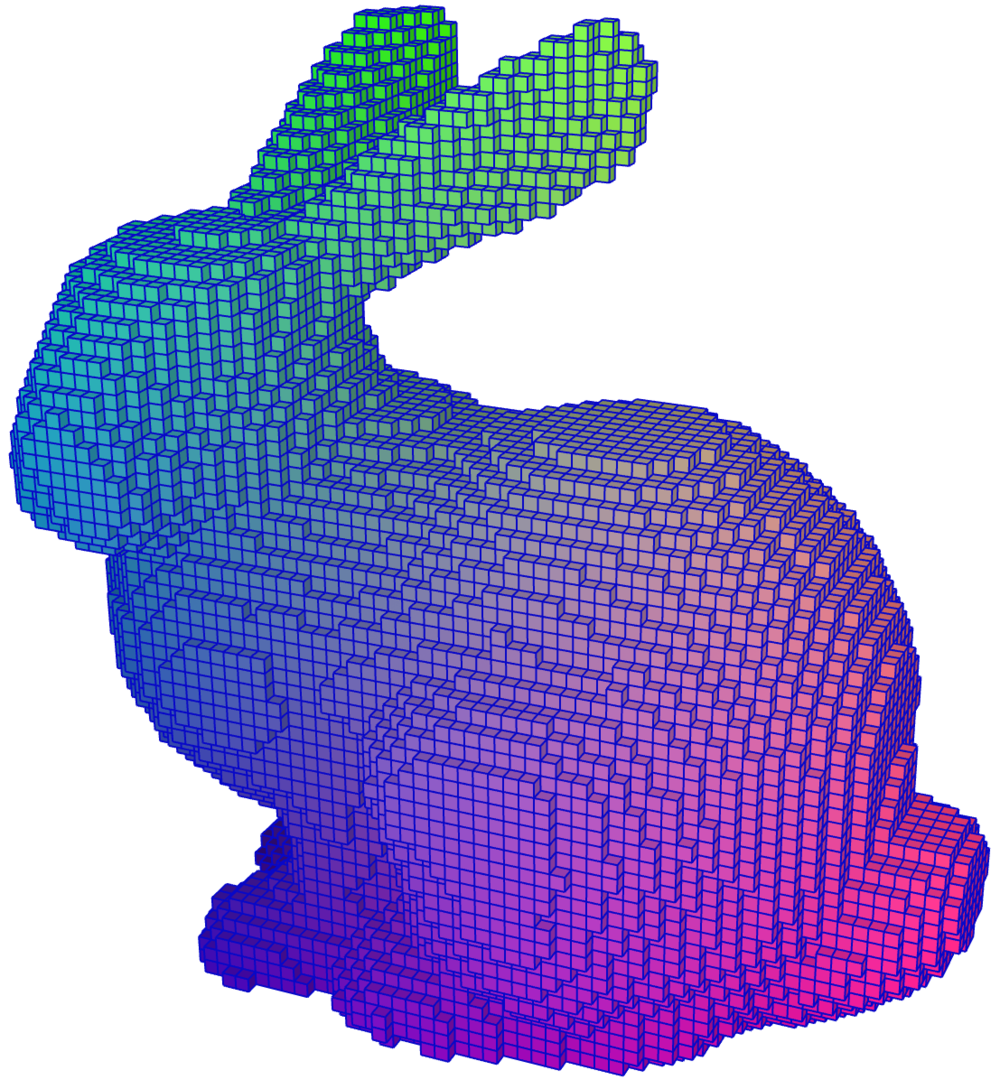
\includegraphics[width=0.3\textwidth]{images/voxel_bunny_borders.png}
        \caption{Voxelization of a 3D asset used with the mesh walking technique. 3D model (left) and voxelized model (right). 
        }
        \label{fig:unity-voxelized}
\end{figure}
